\documentclass[11pt,a4paper]{article}

\usepackage[margin=1in, paperwidth=8.3in, paperheight=11.7in]{geometry}
\usepackage{amsfonts}
\usepackage{amsmath}
\usepackage{amssymb}
\usepackage{color}
\usepackage{enumerate}
\usepackage{enumitem}
\usepackage{fancyhdr}
\usepackage[none]{hyphenat}  % Don't hyphen break words at line breaks
\usepackage[latin1]{inputenc}
\usepackage{listings}
\usepackage{stmaryrd}
\usepackage{tikz}
\usetikzlibrary{shapes,arrows,positioning}

% Setup lstlisting
\lstset{language=Haskell, mathescape=true, showstringspaces=false}

%Define tikz node shapes
\tikzstyle{op} = [rectangle, draw, text width=2em, text centered, minimum height=2em]
\tikzstyle{var} = [regular polygon, regular polygon sides=3, text centered, text width=1.2em, inner sep=0pt, draw]

\begin{document}

\pagestyle{fancy}
\setlength\parindent{0pt}
\allowdisplaybreaks

% Counters
\newcounter{definition}[section]
\newcounter{example}[section]
\newcounter{notation}[section]
\newcounter{proof}[section]
\newcounter{proposition}[section]
\newcounter{remark}[section]
\newcounter{theorem}[section]

% enumerate uses roman
\setlist[enumerate,1]{label=\roman*)}

% commands
\newcommand{\eg}{\textit{e.g.} }
\newcommand{\EG}{\underline{E.G.} - }
\newcommand{\ie}{\textit{i.e.} }
\newcommand{\IE}{\underline{I.E.} - }
\newcommand{\NB}{\underline{N.B.} - }
\newcommand\doubleplus{+\kern-1.3ex+\kern0.8ex} % ++

\newcommand{\notation}[1]{\stepcounter{notation} \textbf{Notation \arabic{section}.\arabic{notation}\ - }\textit{#1}\\}
\newcommand{\proof}[1]{\stepcounter{proof} \textbf{Proof \arabic{section}.\arabic{proof}\ - }\textit{#1}\\}
\newcommand{\proposition}[1]{\stepcounter{proposition} \textbf{Proposition \arabic{section}.\arabic{proposition}\ - }\textit{#1}\\}
\newcommand{\Proposition}[1]{\stepcounter{proposition} \textbf{Proposition \arabic{section}.\arabic{proposition}\ - }\textit{#1}}
\newcommand{\theorem}[1]{\stepcounter{theorem} \textbf{Theorem\arabic{section}.\arabic{theorem}\ - }\textit{#1}\\}

% enviroments
\newenvironment{definition}[1]
	{\stepcounter{definition} \textbf{Definition \arabic{section}.\arabic{definition}\ - }\textit{#1}\\}
	{}
\newenvironment{example}[1]
	{\stepcounter{example} \textbf{Example \arabic{section}.\arabic{example}\ - }\textit{#1}\\}
	{}
\newenvironment{remark}[1]
	{\stepcounter{remark} \textbf{Remark \arabic{section}.\arabic{remark}\ - }\textit{#1}\\}
	{}

\renewcommand{\headrulewidth}{0pt}

% Cover page title
\title{Language Engineering - Reviewed Notes}
\author{Dom Hutchinson}
\date{\today}
\maketitle

% Header
\fancyhead[L]{Dom Hutchinson}
\fancyhead[C]{Language Engineering - Reviewed Notes}
\fancyhead[R]{\today}

\tableofcontents

\textbf{Not Covered}.\\
Below are some \textit{advanced} topics that should only be looked at if happy with everything else
\begin{itemize}
	\item[-]There is an alternative proof technique (to the one discussed in \textbf{2.2}) in \textbf{Chapter 3.4} of the book.
	\item[-]There are extensions to the \textit{While} language which define \textit{Procedures, Locations} \& \textit{Continuations}.
\end{itemize}

% Start of content
\newpage

\section{Syntax}

\subsection{Domain Specific Languages \& Catamorphisms}

\subsubsection{Domain Specific Languages}
This subsection was covered in Teaching Block 1; Lectures 1-4.\\

\begin{definition}{Domain Specific Language}
A \textit{Domain Specific Language} is a programming language that has been design for a specific purpose.\\
\textit{Domain Specific Languages} are not necessarily \textit{Turing Complete}.\\
\EG\textit{SQL} as an example of a \textit{Domain Specific Language} for database management.\\
\NB The term \textit{Domain Specific Languages} is often abbreviated to \textit{DSL}.
\end{definition}\\

\begin{definition}{Embedded Domain Specific Language}
An \textit{Embedded Domain Specific Language} is a \textit{Domain Specific Language} which has been defined within a host language.\\
There are two techniques for embedding a language within the host
\begin{enumerate}
	\item Deep Embedding; and,
	\item Shallow Embedding.
\end{enumerate}
\EG Packages within programming languages can be considered as \textit{Embedded Domain Specific Languages}.\\
\NB The term \textit{Embedded Domain Specific Languages} is often abbreviated to \textit{EDSL}.
\end{definition}\\

\begin{remark}{DSL v EDSL}
When defining a language as an \textit{EDSL} you are restricted by the language you are using, this is not the case for a \textit{DSL} definition.\\
However, when creating a \textit{DSL} definition you have to produce your own parsers \& compilers which consume a lot of time.
\end{remark}

\begin{definition}{Deep Embedding}
In a \textit{Deep Embedding} of an \textit{EDSL} we define the syntax with concrete data types \& the semantics with functions that evaluate these data types.
\end{definition}\\

\begin{definition}{Concrete Data Type}
A \textit{Concrete Data Type} is absolutely defined with only certain inputs \& outputs allowed.\\
\EG Boolean, Integer, Arrays \& Lists.
\end{definition}\\

\begin{example}{Concrete Data Types}
Consider a syntax for adding multiple integers together \eg $3+5$.\\
We have two main features, the values \& the addition symbol, thus we need to define expressions within the constructor.\\
We know the values are strictly integers \& the addition symbol only operates on two values, thus we define
\begin{lstlisting}
data Expr = Var Int
	  | Add Expr Expr
\end{lstlisting}
Then $1+(4+7)\equiv$Add (Var 1) (Add (Var 4) (Var 7)).
\end{example}\\

\begin{definition}{Deep Embedding Semantics}
In a \textit{Deep Embedding} the \textit{Semantics} are defined as functions which evaluate the defined data types.\\
This means they take in a single value of the data type \& produce a single value.
\end{definition}\\

\begin{example}{Deep Embedding Semantics}
Consider define a semantics for the situation describe in \textbf{Example 1.1}.\\
We want to produce an Int value from Expr.\\
We need to define what the evaluation function does for each construction of Expr.\\
We break down the Add constructions \& analyse their sub-structures.
\begin{lstlisting}
eval :: Expr -> Int
eval (Var n)   = n
eval (Add x y) = eval x + eval y
\end{lstlisting}
We then analyse expressions by passing them as inputs to eval.
\end{example}

\begin{definition}{Shallow Embedding}
In a \textit{Shallow Embedding} of an \textit{EDSL} we use the syntax of the host language to define functions that produce results directly.\\
Data types in a \textit{Shallow Embedding} are represented by functions.\\
\NB There is no need for evaluating functions in a \textit{Shallow Embedding}.
\end{definition}\\

\begin{example}{Shallow Embedding}
Consider define a \textit{Shallow Embedding} for an EDSL that adds integers together.\footnote{See \textbf{Example 1.1} \& \textbf{Example 1.2} for the Deep Embedding implementation.}\\
We have two main features, the values \& the addition symbol, thus we need to define functions for each of them.\\
We shall define them to always evaluate to Ints for this example
\begin{lstlisting}
var :: Int -> Int
var n = n
add :: Int -> Int -> Int
add x y = x + y
\end{lstlisting}
Then $1+(4+7)\equiv$add (var 1) (add (var 3) (var 5)).
\end{example}

\subsubsection{Fix \& Catamorphisms}
This subsection was covered in Teaching Block 1; Lecture 4-6.\\

\begin{remark}{Expression Problem}
The \textit{Expression Problem} concerns whether it is possible to extend the syntax \& semantics of a language in a modular way.\\
\ie Can we define a language that is easy to extend both the syntax \& semantics of.\\
\textit{Hard \& Soft Embedding} allow for one of these, but not both.\\
The \textit{Expression Problem} is solved using \textit{Catamorphisms}
\end{remark}

\begin{example}{{\ttfamily{foldr}} - List}
Below is a definition for {\ttfamily{foldr}} to apply a function to a list
\begin{lstlisting}
foldr :: b -> (a->b->b) -> [a] -> b
foldr k f []     = k
foldr k f (x:xs) = f x (foldr k xs)
\end{lstlisting}
\end{example}

\begin{definition}{{\ttfamily{Functor}}}
{\ttfamily{Functor}}s are a class of data types that allow you to work inside the data-structure.\\
{\ttfamily{Functor}} data-types have a function which takes in two inputs: a function \& a {\ttfamily{functor}} data-structure, and then maps the function over the data-structure.\\
In Haskell the \textit{Functor} class is defined as
\begin{lstlisting}
class Functor f where
  fmap :: (a->b) -> f a -> f b
\end{lstlisting}
\end{definition}

\begin{example}{Functor}
Below is an example of how a \textit{Tree} can be instanced as a \textit{Functor}
\begin{lstlisting}
instance Functor Tree where
  fmap f (Leaf x)   = Leaf (f x)
  fmap f (Fork l r) = Fork (fmap f l) (fmap f r)
\end{lstlisting}
Here if the passed value is a \textit{Leaf} then $f$ is applied to its value \& returned.\\
If the passed value is a \textit{Fork} then $f$ is applied to the data-structures below the given \textit{Fork}.
\end{example}\\

\begin{remark}{Recursiveless Datatypes}
Instead of defining data-structures which are defined recursively, in terms of themselves, we can add a parameter that shows where we the recursion would have been \& now tells us the results of previous operations on the data-structure.\\
Doing this breaks data-types down into their smaller constituent parts which are then easier to stitch together.
\end{remark}\\

\begin{example}{Recursiveless Datatypes}
Below is a standard definition of a \textit{List}, without syntactic sugar
\begin{lstlisting}
data List a = Empty
            | Cons a (List a)
\end{lstlisting}
Here we want to change definition of \textit{Cons} to not include \textit{(List a)}.\\
We take an additional parameter for the data-structure which replaces the recursion
\begin{lstlisting}
data ListF a k = EmptyF
               | ConsF a k
\end{lstlisting}
$k$ here tells us results of previous operations on the data-structure.\\
\NB We use renamed the structure to \textit{ListF} to show it can be defined as a functor.
\end{example}\\

\begin{definition}{{\ttfamily{Fix}} - Fixed Point of Types}
The \textit{Fixed Point} of a function is a parameter that when given to the function returns the same value.\\
The \textit{Fix} data-type isolates recursion of all functors to one location, thus generalising recursion.\\
\textit{Fix} takes a functor without its $k$ as a parameter and then stores a copy of itself where the recursive $k$ would go, for future operations to use.\\
\begin{lstlisting}
data Fix f = In (f (Fix f))
\end{lstlisting}
\NB \textit{In :: f (Fix f) $\to$ Fix f}.\\
\NB Considering the above example \textit{Fix} is defined st
\begin{center}
\textit{Fix (ListF a) = In (ListF a (Fix (ListF a))) $\cong$ List a}
\end{center}
\end{definition}

\begin{example}{Fix ListF with 2 Elements}
Below is how we define a list with 2 elements using \textit{Fix}
\begin{center}
\textit{In (ConsF 6 (In (ConsF 4 (In EmptyF))))}
\end{center}
\end{example}

\begin{definition}{{\ttfamily{inop}}}
\textit{inop} is a function that unwraps a \textit{Fix}
\begin{lstlisting}
inop :: Fix f -> f (Fix f)
inop (In x) = x
\end{lstlisting}
\end{definition}

\begin{definition}{Folds}
\textit{Folds} are functions that unwrap data-structures in order to apply a given function to it.\\
\textit{Foldr} is a particular example of a \textit{Fold} which unwraps an \textit{array} left-to-right.\\
\textit{foldr} takes three inputs: a base case; a function; \&, a data-structure to apply it to.\\
The \textit{base case} is returned when the \textit{``Bottom"} of the structure has been reached.
\begin{lstlisting}
foldr :: (a->b->b) -> b -> [a] -> b
foldr f k []     = k
foldr f k (x:xs) = f x (foldr f k xs)
\end{lstlisting}
\NB This is \textit{Foldl} as well.
\end{definition}\\

\begin{definition}{{\ttfamily{cata}} - Catamorphism}
\textit{Catamorphism}s are a generalisation of \textit{folds}.\\
\textit{Algebras} are functions that correspond to replacing the constructors of a data-type with functions.\\
\textit{cata} is a function that applies an algebra to the fixpoint of a value
\begin{lstlisting}
 cata :: Functor f => (f b -> b) -> Fix f -> b
 cata alg     x  = (alg . fmap (cata alg) . inop)x
$\equiv$cata alg (In x) = alg (fmap (cata alg) x)
  where
    alg :: f b -> b
\end{lstlisting}
\end{definition}

\begin{example}{{\ttfamily{cata}}}
Below is an example of how \textit{cata} can be implemented to converted a \textit{Fix (ListF a)} to \textit{List a}.
\begin{lstlisting}
toList :: Fix (ListF a) -> List a
toList x = cata alg x
  where
    alg :: ListF a (List a) -> List a
    alg EmptyF       = Empty
    alg (ConsF x xs) = Cons x xs
\end{lstlisting}
\NB $xs$ denotes the \textit{List a} already generated.\\
Below is an example of how \textit{cata} can be implemented to find the length of a \textit{Fix(ListF a)}
\begin{lstlisting}
toList :: Fix (ListF a) -> Int
toList x = cata alg x
  where
    alg :: ListF a Int -> Int
    alg EmptyF       = 0
    alg (ConsF x y)  = 1 + y
\end{lstlisting}
\NB $y$ marks the length calculated to this point.\\
\end{example}

\subsection{Parsers}
This subsection was covered in Teaching Block 1; Lecture 7-13.

\subsubsection{Composition}

\definition{$:+:$ - Co-Product of Functors}
The \textit{Co-Product of Functors} is used to extend signature functors by composing two functors into one.\\
The \textit{Co-Product of Functors} is defined as
\begin{lstlisting}
data (f:+:g) a = L (f a)
               | R (g a)
\end{lstlisting}
This uses two functors, $f$ \& $g$, to create a single functor $f:+:g$.\\
The \textit{Functor} instance of \textit{:+:} is given as
\begin{lstlisting}
instance (Functor f, Functor g) => Functor (f:+:g)
  where
    fmap f (L x) = L (fmap f x)
    fmap f (R y) = R (fmap f y)
\end{lstlisting}

\example{Co-Product of Functors}
Consider the following functor identity for addition.
\begin{lstlisting}
data ExprF k = ValF Int
             | AddF k k
instance Functor ExprF
  where
    fmap f (ValF n) = ValF n
    fmap f (AddF x y) = AddF (f x) (f y)
\end{lstlisting}
Suppose we want to end to end this include multiplication.\\
We define a multiplication functor identity
\begin{lstlisting}
data MulF k = MulF k k
instance Functor MulF
  where
    fmap f (MulF x y) = MulF (f x) (f y)
\end{lstlisting}
We compose {\ttfamily{ExprF}} \& {\ttfamily{MulF}} simply by using
\begin{lstlisting}
Fix (ExprF:+:MulF)
\end{lstlisting}
This is essential the same as
\begin{lstlisting}
data ExprF = ValF Int
           | AddF ExprF ExprF
           | MulF ExprF ExprF
\end{lstlisting}

\definition{$\nabla$ - Junction of Algebras}
\textit{Junction of Algebras} is used to compose two algebras together.\\
The \textit{Junction of Algebras} is defined as
\begin{lstlisting}
($\nabla$)::(f a$\to$a)$\to$(g a$\to$a)$\to$((f:+:g)a$\to$a)
(flag $\nabla$ galg) (L x) = falg x
(flag $\nabla$ galg) (R y) = falg y
\end{lstlisting}

\example{Junction of Algebras}
Consider the language defined in \textbf{Example 2.1}.\\
We define the following algebras for addition \& multiplication.\\
\begin{lstlisting}
add :: ExprF Int$\to$Int
add (ValF x)  =x
add (AddF x y)=x + y

mul::MulF Int$\to$Int
mul (MulF x y) = x*y
\end{lstlisting}
We can now evaluate {\ttfamily{ExprF}}, using these semantics, using
\begin{lstlisting}
eval :: Fix (ExprF :+: MulF)$\to$Int
eval x = cata (add$\nabla$mul) x
\end{lstlisting}

\subsubsection{Grammars}
% BAckus-Naur Form, Paull's Modified Algorithm

\definition{Backus-Naur Form}
\textit{Backus-Naur Form} is a language used to express the shape of grammars.\\
\textit{Backus-Naur Form} statements use the following symbols\\
\begin{tabular}{c|l}
$\varepsilon$&Empty Strings\\
$<n>$&A non-terminal\\
$``x"$&A terminal\\
$p|q$&A choice between $p$ \& $1$\\
$[e]$&Optional term\\
$(e)$&Group Terms\\
$e*$&0 or more of term $e$\\
$e+$&1 or more of term $e$
\end{tabular}\\
\NB $e+$ is written \textit{somee} \& $e*$ is written \textit{manye}.\\

\example{Backus-Naur Form}
Below is the definition of a digit \& a number using \textit{Backus-Naur Form}
\begin{lstlisting}
<digit> ::= ``0"|``1"|$\dots$|``9"
<num>   ::= <digit> | <digit> <num>
\end{lstlisting}

\definition{Paull's Modified Algorithm}
\textit{Paull's Modified Algorithm} is used to remove recursion from a grammar.\\
Consider a the following grammar
\begin{lstlisting}
A ::=A$\alpha_1$|$\dots$|A$\alpha_n$|$\beta_1$|\dots|$\beta_m$
\end{lstlisting}
Where {\ttfamily{A}} is non-terminal \& $\alpha_i,\beta_J$ are \textit{Backus-Naur Form} expressions.\\
\textit{Paull's Modified Algorithm} states to rewrite this grammar as
\begin{lstlisting}
A ::=$\beta_1$A'|$\dots$|$\beta_m$A'
A'::=$\alpha_1$A'|$\dots$|$\alpha_n$A'|$\varepsilon$
\end{lstlisting}

\example{Paull's Modified Algorithm}
Consider a grammar for addition expressions
\begin{lstlisting}
<expr>::=<expr> ``+" <expr> | <num>
\end{lstlisting}
Here {\ttfamily{A}}={\ttfamily{<expr>}}, $\alpha$={\ttfamily{"+" <expr>}} \& $\beta$={\ttfamily{<num>}}.\\
Applying \textit{Paull's Modified Algorithm} we get
\begin{lstlisting}
<expr> ::=<num><expr'>
<expr'>::=``+"<expr><expr'> | $\varepsilon$
\end{lstlisting}

\subsubsection{Parsers}
% Monadic Parsing

\definition{Parser}
A \textit{Parser} is a function that takes in a list of characters \& returns an array of parsed data \& unconsumed strings.\\
We can define a \textit{Parser} type as
\begin{lstlisting}
newtype Parser a = Parser (String$\to$[(a,String)])
\end{lstlisting}

\proposition{Functor Instance of Parser}
Below is a definition for a {\ttfamily{Functor}} instance for {\ttfamily{Parser}}.\\
This allows us to transform \textit{Parsers} into using different datatypes
\begin{lstlisting}
instance Functor Parser where
  fmap f (Parser px) = Parser ($\lambda$ s$\to$[(f x,s') | (x,s')$\leftarrow$px s])
\end{lstlisting}

\definition{{\ttfamily{parse}}}
In Haskell we define the function {\ttfamily{parse}} which takes in a {\ttfamily{Parser}}\& {\ttfamily{String}}, then applies the parser to the string.\\
{\ttfamily{parse}} is defined by
\begin{lstlisting}
parse :: Parser a$\to$String$\to$[(a,String)]
parse (Parser px) s = px s
\end{lstlisting}

\definition{Trivial Parsers}
There are two trivial parsers: {\ttfamily{fail}}which always fails; and, {\ttfamily{item}} which parses the first {\ttfamily{Char}} off the string.\\
These parsers are defined below
\begin{lstlisting}
fail :: Parser a
fail = Parser ($\lambda$ s$\to$[])
item :: Parser Char
item = Parser (f)
  where
    f []     = []
    f (s:ss) = [(s,ss)]
\end{lstlisting}

\example{{\ttfamily{fail}} \& {\ttfamily{item}}}
Here are examples of {\ttfamily{fail}} \& {\ttfamily{item}} parsing the string {\ttfamily{Hello}}
\begin{lstlisting}
parse fail ``Hello" = []
parse item ``Hello" = [('H',``ello")]
\end{lstlisting}

\definition{{\ttfamily{look}} Parser}
The {\ttfamily{look}} parser allows you to look at the input stream without consuming it
\begin{lstlisting}
look :: Parser String
look = Parser ($\lambda$ s$\to$[(s,s)])
\end{lstlisting}

\definition{{\ttfamily{Monad}} Class}
{\ttfamily{Monad}}s are a class of data-types which allow you to map their internal value, {\ttfamily{>>=}}.\\
{\ttfamily{Monad}}s have a function, {\ttfamily{return}}, which wraps a value as a {\ttfamily{Monad}}.
\begin{lstlisting}
class Monad m where
  (>>=)  :: m a $\to$ (a $\to$ m b) $\to$ m b
  return :: a $\to$ m a
\end{lstlisting}

\definition{{\ttfamily{Monad}} instance for {\ttfamily{Parser}}}
Below is the {\ttfamily{Monad}} instance for {\ttfamily{Parser}}
\begin{lstlisting}
instance Monad Parser where
  return = pure
  (Parser px) >>= f = Parser ($\lambda$s$\to$concat[parse (f x) s' | (x,s')$\leftarrow$px s])
\end{lstlisting}
{\ttfamily{>>=}} allows the function {\ttfamily{f}} to map the value {\ttfamily{x}} parsed by {\ttfamily{px}} to a new value \& producing a new {\ttfamily{Parser}}.\\

\definition{{\ttfamily{satisfy}} Parser}
The {\ttfamily{satisfy}} \textit{parser} takes a function,{\ttfamily{p}}, which maps {\ttfamily{Char}} to {\ttfamily{Bool}}.\\
{\ttfamily{satisfy}} uses the {\ttfamily{item}} parser to parse the first character off a string \& then applies {\ttfamily{p}} to it to decide whether to return the parsed value.
\begin{lstlisting}
satisfy :: (Char$\to$Bool)$\to$Parser Char
satisfy p = item >>= $\lambda$s$\to$ if (p t) then (pure t) else empty
\end{lstlisting}

\example{Parsing a Character}
Below a {\ttfamily{Parser}} is defined which either parses an {\ttfamily{`a'}} or nothing, depending on the first character of the string.
\begin{lstlisting}
parse (satisfy (`a'==)) `abc' = [(`a',`bc')]
parse (satisfy (`a'==)) `xyz' = []
\end{lstlisting}

\subsubsection{Parser Combinators}

\definition{Parser Combinator}
A \textit{Parser Combinator} is a function that takes (several) parsers as inputs \& returns a new parser.\\

\definition{$\langle\$\rangle$ - Type Change Combinator}
$\langle\$\rangle$ is a \textit{Parser Combinator} which takes a function that maps type $a$ to type $b$ \& a \textit{Parser} of type $b$, and then returns a \textit{Parser} of type $b$.
\begin{lstlisting}
($\langle\$\rangle$)::(a$\to$b)$\to$Parser a$\to$Parser b
f $\langle\$\rangle$ px = fmap f px
\end{lstlisting}

\example{$\langle\$\rangle$ - {\ttfamily{digit}} Parser}
Below is a definition that changes the {\ttfamily{item}} to parse an {\ttfamily{Int}} rather than a {\ttfamily{Char}}
\begin{lstlisting}
digit :: Parser Int
digit = digitToInt $\langle\$\rangle$ item
\end{lstlisting}

\definition{$\langle\$$ - Constant Parser}
$\langle\$$ is a \textit{Parser Combinator} that causes a {\ttfamily{Parser}} to always return the same value.
\begin{lstlisting}
($\langle\$$) :: a$\to$Parser b$\to$Parser a
x $\langle\$$ py = fmap (const x) py
\end{lstlisting}

\definition{{\ttfamily{skip}} Parser}
Below is a definition of a parser that always returns an empty array, effectively skipping parsing the rest of the string.
\begin{lstlisting}
skip :: Parser a$\to$Parser ()
skip px = () $\langle\$$ px
\end{lstlisting}

\definition{{\ttfamily{Applicative}} Functors}
The {\ttfamily{Applicative}} \textit{Functors Class} is the class of \textit{Functors} which have two addition functions {\ttfamily{pure}} \& $\langle*\rangle$.\\
{\ttfamily{pure}} which wraps arbitrary values as the {\ttfamily{Functor}} \& $\langle*\rangle$ applies a function to the context of the functor.
\begin{lstlisting}
class (Functor f) => Applicative f where
  pure :: a$\to$f a
  $(\langle*\rangle)$ :: f (a$\to$b)$\to$f a$\to$f b
\end{lstlisting}

\proposition{{\ttfamily{Applicative}} definition of {\ttfamily{Parser}} - $\langle*\rangle$}
Below is the {\ttfamily{Applicative}} instance of {\ttfamily{Parser}}
\begin{lstlisting}
instance Applicative Parser where
  pure x = Parser ($\lambda$s$\to$[(x,s)])
  (Parser pf) $\langle*\rangle$ (Parser px) = Parser ($\lambda$s$\to$[(f x,s")
  					   |(f,s')$\leftarrow$pf s
  					   ,(x,s")$\leftarrow$px s'])
\end{lstlisting}
$\langle*\rangle$ parses a function ,$f$; then parses a value ,$x$; \& then applies the function to the value, $f\ x$.\\
\textit{N.B.} - $\langle*\rangle$ is called \textit{Ap} for apply.\\

\definition{Reverse Ap - $\langle**\rangle$}
The below operator preforms $\langle*\rangle$ in reverse.\\
It parses a value, then parses a function \& then applies the function to the value.
\begin{lstlisting}
(Parser px) $\langle**\rangle$ Parser pf = Parser ($\lambda$s$\to$[(f x,s'')
					| (x,s')$\leftarrow$px s
					, (f,s")$\leftarrow$pf s'])
\end{lstlisting}

\definition{{\ttfamily{Monoidal}} Class}
The {\ttfamily{Monoidal}} \textit{Class} is the class of datatypes which have a neutral value \& a function for appending the two together.
\begin{lstlisting}
class Monoidal f where
  unit :: f ()
  mult :: f a $\to$ f b $\to$ f(a,b)
\end{lstlisting}
\NB The {\ttfamily{Monoidal}} is equivalent to {\ttfamily{Applicative}}.\\

\proposition{{\ttfamily{Monoidal}} definition of {\ttfamily{Parser}}}
Below is the {\ttfamily{Monoidal}} instance of {\ttfamily{Parser}}
\begin{lstlisting}
instance Monoidal Parser where
  unit = Parser ($\lambda$s$\to$[((),s)])
  mult px py = Parser ($\lambda$s$\to$[((x,y),s")
	  		   | (x,s')$\leftarrow$px s
  			   | (y,s")$\leftarrow$py s'])
\end{lstlisting}
{\ttfamily{unit}} is a {\ttfamily{Parser}} that parses noting.\\
{\ttfamily{mult}} is a {\ttfamily{Parser}} that takes a string \& two other {\ttfamily{Parser}}s, then applies the first {\ttfamily{Parser}} to the string \& then applies the second parser to the remainder of the string. {\ttfamily{mult}} returns a tuple of both these values.\\

\definition{$\langle\sim\rangle$ - {\ttfamily{mult}} Combinator}
It is useful to define the {\ttfamily{mult}} combinator from the {\ttfamily{Monoidal}} instance of {\ttfamily{Parser}} as its own binary operation
\begin{lstlisting}
($\langle\sim\rangle$) :: Monoidal f => f a $\to$ f b $\to$ f (a,b)
px $\langle\sim\rangle$ py = mult px py
\end{lstlisting}

\definition{$\langle*$ \& $*\rangle$ - Extracting values from $\langle\sim\rangle$}
The following combinators are defined to extract the first or second values from the parsed tuple from $\langle\sim\rangle$
\begin{lstlisting}
($\langle*$) :: Monoidal f => f a $\to$ f b $\to$ f a
px $\langle*$ py = fst $\langle\$\rangle$ (px $\langle\sim\rangle$)
($*\rangle$) :: Monoidal f => f a $\to$ f b $\to$ f b
px $*\rangle$ py = snd $\langle\$\rangle$ (px $\langle\sim\rangle$)
  where
    fst (x,y) = x
    snd (x,y) = y
\end{lstlisting}
\NB There two additional operators which are equivalent to these $\langle\sim=\langle*$ \& $\sim\rangle=*\rangle$.\\

\definition{{\ttfamily{Alternative}} Class}
The {\ttfamily{Alternative}} \textit{Class} is a subclass of {\ttfamily{Applicative}} of data types which have a neutral element,{\ttfamily{empty}} \& an operator, $\langle|\rangle$, for choosing between two of the same type.
\begin{lstlisting}
class (Applicative f) => Alternative f where
  empty :: f a
  ($\langle|\rangle$)    :: f a $\to$ f a $\to$ f a
\end{lstlisting}

\definition{{\ttfamily{Alternative}} definition of {\ttfamily{Parser}} - $\langle|\rangle$}
Below is the {\ttfamily{Alternative}} instance of {\ttfamily{Parser}}
\begin{lstlisting}
instance Alternative Parser where
  empty = fail
  (Parser px) $\langle|\rangle$ (Parser py) = Parser ($\lambda$s$\to$(px s)$\doubleplus$(py s))
\end{lstlisting}
$\langle|\rangle$ is a combinator which returns a single array contain the result of parsing the same string with two different parsers.\\
\NB {\ttfamily{px}} \& {\ttfamily{py}} must output the same data type from parsing.\\

\definition{{\ttfamily{choice}}}
{\ttfamily{choice}} is a function that extends the $\langle|\rangle$ combinator to allow for more than two parsers as input
\begin{lstlisting}
choice :: [Parser a] $\to$ Parser a
choice pxs = foldr ($\langle|\rangle$) empty pxs
\end{lstlisting}
% <$>,<|>,<*>

\definition{$\langle:\rangle$ - Append Combinator}
$\langle:\rangle$ is a combinator that appends the result of using one {\ttfamily{Parser}} onto the results of using other {\ttfamily{Parser}}s
\begin{lstlisting}
($\langle:\rangle$) :: Parser a $\to$ Parser [a] $\to$ Parser [a]
px $\langle:\rangle$ pxs = (:) $\langle\$\rangle$ px $\langle*\rangle$ pxs
\end{lstlisting}

\definition{\ttfamily{some}}
The {\ttfamily{some}} operation is equivalent to $e+$ from \textit{Backus-Naur Form}.
\begin{lstlisting}
some :: Parser a $\to$ Parser [a]
some px = px $\langle:\rangle$ many px
\end{lstlisting}
This parses one {\ttfamily{Parser}}, {\ttfamily{px}}, and appends this result to the result of {\ttfamily{many px}}.\\

\definition{\ttfamily{many}}
The {\ttfamily{many}} operation is equivalent to $e*$ from \textit{Backus-Naur Form}.
\begin{lstlisting}
many :: Parser a $\to$ Parser [a]
many px = some px  $\langle|\rangle$ pure
\end{lstlisting}
This returns the result of {\ttfamily{some px}}, if no such result exists then it returns {\ttfamily{empty}}

\remark{Summary of Combinator Operations}
\begin{tabular}{ll}
$\langle\$\rangle$&Changes type of a {\ttfamily{Parser}}.\\
$\langle\$$&Makes a {\ttfamily{Parser}} always return the same value.\\
$\langle*\rangle$&Uses one {\ttfamily{Parser}} to parse a function  \& another {\ttfamily{Parser}} to parse a value,\\
&then applies the function to the value.\\
$\langle*\rangle$&Uses one {\ttfamily{Parser}} to parse a value\& another {\ttfamily{Parser}} to parse a function,\\
&then applies the function to the value.\\
$\langle\sim\rangle$&Uses one {\ttfamily{Parser}} to parse a string\& another {\ttfamily{Parser}} to parse the remaining string,\\
&then returns a tuple of the two parsed value \& the remaining string.\\
$\langle\sim$ or $\langle*$& Performs $\langle\sim\rangle$ but returns only the result of the \underline{first} {\ttfamily{Parser}}.\\
$\sim\rangle$ or $*\rangle$& Performs $\langle\sim\rangle$ but returns only the result of the \underline{second} {\ttfamily{Parser}}.\\
$\langle|\rangle$&Applies two {\ttfamily{Parser}}s to the same string \& returns a single array with both results.\\
$\langle:\rangle$&Appends the result of using one {\ttfamily{Parser}} onto the results of using multiple other {\ttfamily{Parser}}s.
\end{tabular}

\subsection{Abstract Syntax}
% Abstract Syntax Trees
% A Free Monad provides an abstract syntax tree & a way to intrepet that tree

\definition{Syntax Tree}
A \textit{Syntax Tree}s are used to describe dependency in a syntax.\\
Squares are used to signify operations \& triangles to signify variables.\\
No shape signifies a constant value.\\
The children of a node show the values that are dependent upon it, only an operation will have dependants.\\

\example{Syntax Tree}
Below is a \textit{Syntax Tree} for $(x+y)+z$.\\
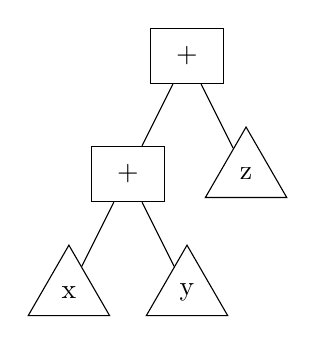
\begin{tikzpicture}
\node[op] {+}
	child { node[op] {+}
		child { node[var] {x} }
		child { node[var] {y} }
	}
	child { node[var] {z} };
\end{tikzpicture}\\
Note that both $+$s are denoted as operations, while $x,y,z$ are denoted as variables.\\

\subsubsection{The Free Monad}

\definition{{\ttfamily{Free}} Monad}
The \textit{Free Monad}, {\ttfamily{Free f a}}, is used to produce syntax trees who nodes operations are defined by {\ttfamily{f}} and whose variables are all of type {\ttfamily{a}}.
\begin{lstlisting}
data Free f a = Var a
              | Op (f (Free f a))
\end{lstlisting}

\example{{\ttfamily{Free}} Monad}
The syntax tree from \textbf{Example 3.1} can be defined, using {\ttfamily{AddF}} from \textbf{Example 2.1}, as
\begin{lstlisting}
Op(AddF (Op (AddF (Var "x") (Var "y"))) (Var "z"))
\end{lstlisting}

\definition{Generator \& Algebra}
There are two stages to interpreting {\ttfamily{Free}} trees
\begin{enumerate}[label=\roman*)]
	\item \textit{Generator}. Changing variables into a value; \&,
	\item \textit{Algebra}. Evaluating the operations.
\end{enumerate}

\definition{{\ttfamily{Functor}} instance of {\ttfamily{Free}}}
Defining a {\ttfamily{Functor}} of instance of {\ttfamily{Free}} allows us to replace variables with their values, since we can inspect within the tree.\\
\NB This is the \textit{Generator} stage of interpreting {\ttfamily{Free}} trees.
\begin{lstlisting}
instance Functor f => Functor (Free f) where
  fmap f (Var x) = Var (f x)
  fmap f (Op op) = Op (fmap (fmap f) op
\end{lstlisting}

\definition{{\ttfamily{Monad}} instance of {\ttfamily{Free}}}
We define a {\ttfamily{Monad}} instance of {\ttfamily{Free}} in order to perform \textit{substitution}
\begin{lstlisting}
instance Functor f => Monad (Free f) where
  return x = Var x
  (Var x) >>= f = f x
  (Op op) >>= f = Op (fmap (>>= f) op)

\end{lstlisting}

\definition{{\ttfamily{extract}}}
We define the recursive function {\ttfamily{extract}} to evaluate operations within a {\ttfamily{Free}} tree.\\
This is the \textit{Algebra} stage of interpreting {\ttfamily{Free}} trees.
\begin{lstlisting}
extract :: Functor f => (f b$\to$ b)$\to$Free f b$\to$b
extract alg (Var x) = x
extract alg (Op op) = alg (fmap (extract alg) op)
\end{lstlisting}
\NB We define the use of {\ttfamily{b}} here since this function takes in the result of using {\ttfamily{Free}} functor

\definition{\ttfamily{eval}}
The {\ttfamily{eval}} function combines the \textit{Generating} \& \textit{Algebra} stages of interpreting {\ttfamily{Free}} trees, producing a single value in the end.
\begin{lstlisting}
eval :: Functor f => (f b$\to$b)$\to$(a$\to$b)$\to$Free f a$\to$b
eval alg gen t = (extract alg)$\cdot$(fmap gen) t
\end{lstlisting}

\subsubsection{Additional Syntax}

\definition{\ttfamily{Fail}}
{\ttfamily{Fail}} is a syntax for failure
\begin{lstlisting}
data FailF k = FailF
instance Functor FailF where
  fmap f FailF = FailF
\end{lstlisting}
We need to define a {\ttfamily{Functor}} instance of {\ttfamily{Fail}} to show that no computations follow a failure

\example{\ttfamily{Fail}}
Consider define a language with division in it, {\ttfamily{DivF}}.\\
We need to consider the case when dividing by $0$. No value will be computed so we need to signify that the failure has occurred.\\
We do so by allowing failure in the the \textit{Algebra}
\begin{lstlisting}
alg :: DivF (Free FailF Double)$\to$Free FailF Double
alg (DivF (Var x) (Var 0)) = Op FailF
alg (DivF (Var x) (Var y)) = Var (x/y)
alg _                      = Op FailF
\end{lstlisting}
\NB this algebra also fails when an incorrect {\ttfamily{Free}} shape is passed.\\

\definition{Substitution}
\textit{Substitution} allows us to replace part of an expression with another expression.\\
The follow syntax is used to show that all occurrences of {\ttfamily{x}} in expression {\ttfamily{e}} should be replaced with a new expression {\ttfamily{e'}}.
\begin{lstlisting}
e[x$\mapsto$e']
\end{lstlisting}
The {\ttfamily{>>=}} operation is used for substitution. {\ttfamily{e >>= f}} binds the substitution defined by {\ttfamily{f}} to the syntax tree/expression {\ttfamily{e}}.\\

\definition{\ttfamily{Or}}
We define the {\ttfamily{Or}} data-type to denote when we have a choice between two operations.\\
\begin{lstlisting}
data Or k=Or k k
instance Functor Or where
  fmap f (Or x y) = Or (f x) (f y)
\end{lstlisting}
\NB We define a {\ttfamily{Functor}} instance for {\ttfamily{Or}} so that it can be used in {\ttfamily{Free}} trees.\\

\definition{\ttfamily{once}}
We define the function {\ttfamily{once}} to make choices about which computation stored in {\ttfamily{Or}}.\\
{\ttfamily{once}} simply picks the first available computation.
\begin{lstlisting}
once :: Free Or a$\to$Maybe a
once t = eval alg gen t
  where
    gen x = Just x
    alg (Or Nothing y)  = y
    alg (Or (Just x) _) = Just x
\end{lstlisting}
\NB We define using {\ttfamily{y}} rather than {\ttfamily{Just y}} so that when both values are {\ttfamily{Nothing}}

\definition{\ttfamily{Nondet}}
\textit{Non-Deterministic} computations provide a choice between two computations.\\ 
We use $p\square q$ to denote the operation that offers a choice between $p$ \& $q$.
\begin{lstlisting}
type Nondet a = (Fail :+: Or) a
\end{lstlisting}
This defines a non-deterministic data-type which allows for failure.\\
\NB {\ttfamily{Fail :+: Or}} means we have {\ttfamily{(L Fail)}} \& {\ttfamily{(R (Or x y))}} as structures.\\

\example{\ttfamily{list}}
Below is define a function {\ttfamily{list}} which traverses a {\ttfamily{Free}} tree with {\ttfamily{Nondet}} operations \& returns an array of all non-failed value
\begin{lstlisting}
list :: Free Nondet a$\to$[a]
list t = eval alg gen t
  where
    gen x = [x]
    alg (L Fail) = []
    alg (R (Or x y)) = x++y
\end{lstlisting}

\definition{\ttfamily{Alt}}
\textit{Alternation} is an alternative way to represent \textit{Non-Deterministic} operations, by pairing values with booleans.\\
The idea being we pass {\ttfamily{True}} when we want the first value\& {\ttfamily{False}}  when we want the second.
\begin{lstlisting}
data Alt k = Alt (Bool$\to$k)
instance Functor Alt where
  fmap f (Alt k) = Alt (f$\cdot$k)
\end{lstlisting}
This allows us to redefine {\ttfamily{Nondet}}
\begin{lstlisting}
type Nondet' a = (Fail :+: Alt) a
\end{lstlisting}

\example{{\ttfamily{list}} with new {\ttfamily{Nondet'}}}
Below we define {\ttfamily{list}} using {\ttfamily{Nondet'}}, it still collects all non-failed values
\begin{lstlisting}
list :: Free Nondet' a$\to$[a]
list t = eval alg gen t
  where
    gen x = [x]
    alg (L Fail) = []
    alg (R (Alt k)) = (k True) ++ (k False)
\end{lstlisting}

\definition{\ttfamily{State}}
A \textit{Stateful} computation has two particular operations {\ttfamily{Get}} \& {\ttfamily{Put}}
\begin{lstlisting}
data State s k = Put s k
               | Get (s$\to$k)
\end{lstlisting}
{\ttfamily{Put s k}} will put the value {\ttfamily{s}} into the state before continuing the computation {\ttfamily{k}}.\\
{\ttfamily{Get f}} will only continue {\ttfamily{f}} is given a variable of type {\ttfamily{s}}.\\

\example{\ttfamily{evalState}}
We define {\ttfamily{evalState}} to evaluate {\ttfamily{Free}} trees with {\ttfamily{State s}} operations
\begin{lstlisting}
evalState :: Free (State s) a$\to$(s$\to$(a,s))
evalState t = eval alg gen t
  where
    gen x s = (x,s)
    alg (Put s' k) = ($\lambda$s$\to$k s')
    alg (Get k)    = ($\lambda$s$\to$k s s) // $1^{st}$ s is state that generates program
                                    $2^{nd}$ s is state passed on to future program
\end{lstlisting}

\newpage
\section{Semantics}

\remark{Semantics}
\textit{Semantics} assign meaning to expressions. They can be considered to assign meaning to \textit{Abstract Syntax Trees}.\\
\NB A \textit{Semantic Function} can be considered as a map from syntax to semantics.\\

\example{Semantic Function}
Defined below is a function that assigns \textit{Semantic} meaning to a binary number, by mapping it to its decimal value
\[\begin{array}{l}
\mathcal{N}:Num\to\mathbb{Z}\\
\mathcal{N}\llbracket 0\rrbracket=0\\
\mathcal{N}\llbracket 1\rrbracket=1\\
\mathcal{N}\llbracket  n0\rrbracket=2*\mathcal{N}\llbracket  n\rrbracket\\
\mathcal{N}\llbracket  n1\rrbracket=1+2*\mathcal{N}\llbracket  n\rrbracket
\end{array}\]

\definition{Program State}
A \textit{Program State} is an injective map from variables to integers.
$$State=Var\to\mathbb{Z}$$
A \textit{Program State} is used with a \textit{Semantic Function} to find the result of the \textit{Semantic Function} for different values of the variables. (The \textit{Program State} is updated throughout the execution of the \textit{Semantic Function}).\\
\NB See \textbf{0. Reference} for notation.\\

\definition{Semantic Equivalence}
Two statements, $a \& b$, are semantically equivalent iff $\mathcal{F}\llbracket  a\rrbracket s=\mathcal{F}\llbracket  b\rrbracket\ \forall\ s\in State$, for an appropriate $\mathcal{F}$.\\

\definition{Arithmetic Semantic Function}
Defined below is a \textit{Semantic Function} for arithmetic expressions
\[\begin{array}{lcl}
\mathcal{A}&:&Aexp\to(State\to\mathbb{Z})\\
\mathcal{A}\llbracket  n\rrbracket s&=&s\ x\\
\mathcal{A}\llbracket  a_1+a_2\rrbracket s&=&\mathcal{A}\llbracket  a_1\rrbracket s+\mathcal{A}\llbracket  a_2\rrbracket s\\
\mathcal{A}\llbracket  a_1-a_2\rrbracket s&=&\mathcal{A}\llbracket  a_1\rrbracket s-\mathcal{A}\llbracket  a_2\rrbracket s\\
\mathcal{A}\llbracket  a_1*a_2\rrbracket s&=&\mathcal{A}\llbracket  a_1\rrbracket s*\mathcal{A}\llbracket  a_2\rrbracket s
\end{array}\]

\definition{Boolean Semantic Function}
Defined below is a \textit{Semantic Function} for boolean expressions
\[\begin{array}{lcl}
\mathcal{B}&:&Bexp\to(State\to T)\\
\mathcal{B}\llbracket  true\rrbracket s&=&tt\\
\mathcal{B}\llbracket  false\rrbracket s&=&ff\\
\mathcal{B}\llbracket  a_1=a_2\rrbracket s&=&\begin{cases}tt&\mathcal{A}\llbracket  a_1\rrbracket s=\mathcal{A}\llbracket  a_2\rrbracket s\\ff&\mathcal{A}\llbracket  a_1\rrbracket s\neq\mathcal{A}\llbracket  a_2\rrbracket s\end{cases}\\
\mathcal{B}\llbracket  a_1\leq a_2\rrbracket s&=&\begin{cases}tt&\mathcal{A}\llbracket  a_1\rrbracket s\leq\mathcal{A}\llbracket  a_2\rrbracket s\\ff&\mathcal{A}\llbracket  a_1\rrbracket s>\mathcal{A}\llbracket  a_2\rrbracket s\end{cases}\\
\mathcal{B}\llbracket  \neg b\rrbracket s&=&\begin{cases}tt&\mathcal{B}\llbracket  b\rrbracket s=tt\\ff&\mathcal{B}\llbracket  b\rrbracket s=ff\end{cases}\\
\mathcal{B}\llbracket  b_1\wedge b_2\rrbracket s&=&\begin{cases}tt&\mathcal{B}\llbracket  b_1\rrbracket s=tt\ \mathrm{and}\ \mathcal{B}\llbracket  b_2\rrbracket s=tt\\ff&\mathcal{B}\llbracket  b_1\rrbracket s=ff\ \mathrm{or}\ \mathcal{B}\llbracket  b_2\rrbracket s=ff\end{cases}
\end{array}\]
\NB $T=\{tt,ff\}$.\\

\definition{Free Variables of Semantics}
The \textit{Free Variables} of an arithmetic expression are the set of variables occurring within it.\\
\eg The free variables of $(x+y)*y$ are $\{x,y\}$.\\

\definition{Substitutions of Semantics}
\textit{Substitution} in semantics is the process of replacing a variable with an expression.\\
Suppose we have an expression $a$ \& want to replace all occurrences of variable $y$ with the expression $a_0$ we write
$$a[y\mapsto a_0]$$
Formally we define substitution as
\[\begin{array}{rcl}
n[y\mapsto a_0]&=&n\\
x[y\mapsto a_0]&=&\begin{cases}a_0&x=y\\x&x\neq y\end{cases}\\
(a_1+a_2)[y\mapsto a_0)&=&(a_1[y\mapsto a_0])+(a_2[y\mapsto a_0])\\
(a_1-a_2)[y\mapsto a_0)&=&(a_1[y\mapsto a_0])-(a_2[y\mapsto a_0])\\
(a_1*a_2)[y\mapsto a_0)&=&(a_1[y\mapsto a_0])*(a_2[y\mapsto a_0])\\
(s[y\mapsto v])x&=&\begin{cases}v&x=y\\s\ x&x\neq y\end{cases}
\end{array}\]

\subsection{Operational Semantics}

\remark{Operational Semantics}
\textit{Operational Semantics} is concerned with how a computation is executed, not just the result.\\

\definition{Configuration}
There are two types of \textit{Configuration}
\begin{enumerate}[label=\roman*)]
	\item An \textit{intermediate configuration} - $\langle x,\sigma\rangle$ where $x$ is a syntactic expression \& $\sigma$ is a state.
	\item A \textit{Final Configuration} - $y$ a syntactic value.
\end{enumerate}

\notation{Derivation Tree}
Let $\delta_i$ \& $\gamma_i$ be configurations st $\delta_i\to\gamma_i$.\\
Let $\delta_0\to\gamma_0$ be the result we want to show, this is called the \textit{Conclusion}.\\
We need to derive other configurations to prove that this holds, these are called \textit{Premises}.
$$\dfrac{\delta_1\to\gamma_1\dots\delta_n\to\gamma_n}{\delta_0\to\gamma_0}$$
\NB More layers can be added when a \textit{Premises} needs to be proved.

\remark{Rule v Axiom}
\textit{Rules} have one conclusion \& at least one premise.\\
\textit{Axiomata} have no premises.\\
\NB In \textbf{Definition 2.8} $[skip_{ns}]$ is an \textit{axiom} \& $[comp_{ns}]$ is a \textit{rule}.

\subsubsection{Natural Operational Semantics}

\remark{Natural Operational Semantics}
\textit{Natural Operational Semantics} is concerned with the relationship between the initial state \& final state.\\
Thus the transition relation, $\to$, specifies the relationship between initial \& final state for each statement.\\
$\langle S,s\rangle\to s'$ means that when statement $S$ is applied to state $s$ it results in state $s'$.\\
\NB This is often referred to as the \textit{Big Step}.\\

\definition{Rules \& Axioms of Natural Semantics}
\begin{tabular}{ll}
$[skip_{ns}]$&$\overline{\langle skip,\sigma\rangle\to\sigma}$\\
$[ass_{ns}]$&$\overline{\langle x:=a\rangle\to\sigma[x\mapsto\mathcal{A}\llbracket  a\rrbracket\sigma]}$\\
$[comp_{ns}]$&$\dfrac{\langle S_1,s\rangle\to s',\ \langle S_2,s'\rangle\to s''}{\langle S_1;S_2,s\rangle\to s''}$\\
$[if_{ns}^{tt}]$&$\dfrac{\langle S_1,s\rangle\to s'}{\langle if\ b\ then\ S_1\ else\ S_2,s\rangle\to s'}$ if $\mathcal{B}\llbracket  b\rrbracket s=tt$\\
$[if_{ns}^{ff}]$&$\dfrac{\langle S_2,s\rangle\to s'}{\langle if\ b\ then\ S_1\ else\ S_2,s\rangle\to s'}$ if $\mathcal{B}\llbracket  b\rrbracket s=ff$\\
$[while_{ns}^{tt}]$&$\dfrac{\langle S,s\rangle\to s',\ \langle while\ b\ do\ S,s'\rangle\to s''}{\langle while\ b\ do\ S,s\rangle\to s''}$ if $\mathcal{B}\llbracket  b\rrbracket=tt$\\
$[while_{ns}^{tt}]$&$\langle while\ b\ do\ S,s\rangle\to s$ if $\mathcal{B}\llbracket  b\rrbracket=ff$
\end{tabular}\\

\definition{Semantic Function, $\mathcal{S}_{ns}$}
This \textit{Semantic Function} is a partial function which summarises the \textit{meaning} of \textit{Natural Semantics} statements
\[\begin{array}{rcl}
\mathcal{S}_{ns}&:&Stm\to(State\hookleftarrow State)\\
\mathcal{S}_{ns}\llbracket  S\rrbracket\sigma&=&\begin{cases}\sigma'&\langle S,\sigma\rangle\to\sigma'\\\bot&\mathrm{otherwise}\end{cases}
\end{array}\]
\NB $\mathcal{S}_{ns}\llbracket  S\rrbracket=\mathcal{S}_{sos}\llbracket  S\rrbracket\ \forall\ S$.\\

\definition{Types of Statement}
There are two types of statements
\begin{enumerate}[label=\roman*)]
	\item \textit{Terminating} iff $\exists\ s'\ st\ \langle S,s\rangle\to s'$
	\item \textit{Looping} iff $\nexists\ s'\ st\ \langle S,s\rangle\to s'$
\end{enumerate}
A statement \textit{always terminates} if it is terminating $\forall\ s$.\\
A statement \textit{always loops} if it loops $\forall\ s$.\\

\definition{Equivalence}
Two statements are equivalent if
$$\forall\ s \langle S_1,s\rangle\to s'\ and\ \langle S_2,s\rangle\to s'$$

\definition{Deterministic}
A statement $S$ is \textit{Deterministic} if
$$\forall\ s,s',s''\ if\ \langle S,s\rangle\to s'\ \&\ \langle S,s\rangle\to s''\implies s'=s''$$

\subsubsection{Structural Operational Semantics}

\remark{Structural Operation Semantics}
\textit{Structural Operation Semantics} is concerned with the individual steps of execution.\\
The transition relation, $\Rightarrow$, expresses the first step of the execution of a statement.\\
$\langle S,s\rangle\Rightarrow\langle S',s'\rangle$ means that when executing the first step of statement $S$ on state $s$ results in statement $S'$ \& state $s'$.\\

\definition{Rules \& Axiomata of Structural Semantics}
\begin{tabular}{ll}
$[skip_{sos}]$&$\langle x:= a,s\rangle\Rightarrow s[x\mapsto\mathcal{A}\llbracket  a\rrbracket s]$\\
$[ass_{sos}]$&$\langle skip,s\rangle\Rightarrow s$\\
$[comp_{sos}^1]$&$\dfrac{\langle S_1,s\rangle\Rightarrow\langle S_1',s'\rangle}{\langle S_1;S_2,s\rangle\Rightarrow\langle S_1';S_2,s'\rangle}$\\
$[comp_{sos}^2]$&$\dfrac{\langle S_1,s\rangle\Rightarrow s'}{\langle S_1;S_2,s\rangle\Rightarrow\langle S_2,s'\rangle}$\\
$[if_{sos}^{tt}]$&$\langle\ if\ b\ then\ S_1\ else\ S_2,s\rangle\Rightarrow\langle S_1,s\rangle$ if $\mathcal{B}\llbracket  b\rrbracket=tt$\\
$[if_{sos}^{ff}]$&$\langle\ if\ b\ then\ S_1\ else\ S_2,s\rangle\Rightarrow\langle S_2,s\rangle$ if $\mathcal{B}\llbracket  b\rrbracket=ff$\\
$[while_{sos}]$&$\langle while\ b\ do\ S,s\rangle\Rightarrow\langle if\ b\ then\ (S;\ while\ b\ do\ S)\ else\ skip,s\rangle$
\end{tabular}\\

\definition{Semantic Function, $\mathcal{S}_{sos}$}
This \textit{Semantic Function} is a partial function which summarises the \textit{meaning} of \textit{Operational Semantics} statements
\[\begin{array}{rcl}
\mathcal{S}_{sos}&:&Stm\to(State\hookleftarrow State)\\
\mathcal{S}_{sos}\llbracket  S\rrbracket s&=&\begin{cases}s'&\langle S,s\rangle\Rightarrow^*s'\\\bot&\mathrm{otherwise}\end{cases}
\end{array}\]
\NB $\mathcal{S}_{ns}\llbracket  S\rrbracket=\mathcal{S}_{sos}\llbracket  S\rrbracket\ \forall\ S$.\\

\definition{Stuck Configuration}
A \textit{Configuration} $\langle S,s\rangle$ is \textit{stuck} if
$$\nexists\ S',s'\ st\ \langle S,s\rangle\Rightarrow\langle S',s'\rangle$$

\definition{Types of Derivation Sequence}
Let $\gamma_i=\langle S_i,s_i\rangle$ be configurations.\\
There are two types of \textit{Derivation Sequence}
\begin{enumerate}[label=\roman*)]
	\item \textit{Finite Sequence} iff $\exists\ k\in\mathbb{N}$ st $\gamma_k$ is a terminating or stuck configuration of $\gamma_0$.
	\item \textit{Infinite Sequence} if no such $k$ exists.
\end{enumerate}
\NB A configuration terminates iff it derives a finite sequence. A configuration loops iff it derives an infinite sequence.

\subsubsection{Natural Operational Semantics v Structural Operational Semantics}

\Proposition{Summary of Proof that $\mathcal{S}_{ns}\llbracket  S\rrbracket=\mathcal{S}_{sos}\llbracket  S\rrbracket\ \forall\ S$}
\begin{enumerate}[label=\roman*)]
	\item Proof by \textit{Induction on the Shape of Derivation Trees} that for each derivation tree in the natural semantics there is a corresponding finite derivation sequence in the structural operational semantics.
	\item Proof by \textit{Induction on the Length of Derivation Sequences} that for each finite derivation sequence in the structural operational semantics there is a corresponding derivation tree in the natural semantics.
\end{enumerate}

\proposition{Abnormal Termination}
In a natural semantics we cannot distribugish between looping \& abnormal termination (\ie {\ttfamily{abort}}.\\
In structural semantics looping is reflected by infinite derivation sequences and abnormal termination by finite derivation sequences ending in a stuck configuration.\\

\proposition{Non-Determinism}
In a natural semantics non-determinism will suppress looping, if possible.\\
In a structural semantics non-determinism does not suppress looping.\\

\proposition{Parallelism}
In a natural semantics the execution of the immediate constituents is atomic entity so we cannot express interleaving computations.\\
In a structural operation semantics we concentrate on the small steps of the computation, so can easily express interleaving.

\subsection{Provably Correct Implementation}

\remark{Correctness of a Language}
Defining a formal specification for the semantics of a language using one the semantic forms defined in this unit allows us to prove the correctness of its implementation.\\
Here the correctness of \textit{While} is proved by define an \textit{Operational Semantics} for it, which can then be executed by an \textit{Abstract Machine}.\\

\proposition{Process of Proving Correctness}
The correctness result states that if we can
\begin{itemize}
	\item[-] Translate a program into code;
	\item[-] Execute the code on the abstract machine; \&
	\item[-] Get the same result as specified by the semantic functions $S_{ns}$ \& $S_{sos}$
\end{itemize}
then the language is correct.\\

\definition{Abstract Machine}
An \textit{Abstract Machine} is a theoretical model of a computer.\\
\textit{Abstract Machine}s use configurations of the form $\langle c,e,s\rangle$ where
\begin{itemize}
	\item[-] $c$ is the code to be executed;
	\item[-] $e$ is the evaluation stack which evaluates arithmetic \& boolean expression; and
	\item[-] $s$ is the storage of values for variables.
\end{itemize}

\definition{Instructions for Abstract Machine}
The \textit{Instructions} for the \textit{Abstract Machine} are given by the following abstract syntax\\
\begin{tabular}{lcl}
inst&::=&PUSH-$n$ \textbar ADD \textbar MULT \textbar SUB\\
&\textbar&TRUE \textbar FALSE \textbar EQ \textbar LE \textbar AND \textbar NEG\\
&\textbar&FETCH-$x$ \textbar STORE-$x$\\
&\textbar& NOOP \textbar BRANCH($c,c$) \textbar LOOP($c,c$)\\
c&::=& $\varepsilon$ \textbar inst:$c$
\end{tabular}\\

\definition{Terminal Configuration}
A \textit{Configuration}, $\langle c,e,s\rangle$ is \textit{terminal} if it has the form $\langle\varepsilon,e,s\rangle$ (\ie It's code component is empty).\\

\definition{Transition Relation, $\rhd$}
The transition relation $\rhd$ shows the result of \textit{one-step} of execution.$\langle c,e,s\rangle\rhd\langle c',e',s'\rangle$ means $\langle c,e,s\rangle$ becomes $\langle c',e',s'\rangle$ after executing the first expression in the stack.\\

\definition{Definitions of Instructions}
\begin{tabular}{lcll}
$\langle$PUSH-$n:c,e,s\rangle$&$\rhd$&$\langle c,\mathcal{N}[[n\rrbracket:e,s\rangle$\\
$\langle$ADD$:c,z_1:z_2:e,s\rangle$&$\rhd$&$\langle c,(z_1+z_2):e,s\rangle$&if $z_1,z_2\in\mathbb{Z}$\\
$\langle$MULT$:c,z_1:z_2:e,s\rangle$&$\rhd$&$\langle c,(z_1\times z_2):e,s\rangle$&if $z_1,z_2\in\mathbb{Z}$\\
$\langle$SUB$:c,z_1:z_2:e,s\rangle$&$\rhd$&$\langle c,(z_1-z_2):e,s\rangle$&if $z_1,z_2\in\mathbb{Z}$\\
$\langle$TRUE$:c,e,s\rangle$&$\rhd$&$\langle c,tt:e,s\rangle$\\
$\langle$FALSE$:c,e,s\rangle$&$\rhd$&$\langle c,ff:e,s\rangle$\\
$\langle$EQ$:c,z_1:z_2:e,s\rangle$&$\rhd$&$\langle c,(z_1=z_2):e,s\rangle$&if $z_1,z_2\in\mathbb{Z}$\\
$\langle$LE$:c,z_1:z_2:e,s\rangle$&$\rhd$&$\langle c,(z_1\leq z_2):e,s\rangle$&if $z_1,z_2\in\mathbb{Z}$\\
$\langle$AND$:c,t_1:t_2:e,s\rangle$&$\rhd$&$\langle c,(t_1\wedge t_2):e,s\rangle$&if $z_1,z_2\in\mathbb{Z}$\\
$\langle$NEG$:c,t_1:t_2:e,s\rangle$&$\rhd$&$\langle c,(t_1\neq t_2):e,s\rangle$&if $z_1,z_2\in\mathbb{Z}$\\
$\langle$FETCH$-x:c,e,s\rangle$&$\rhd$&$\langle c,(s\ x):e,s\rangle$\\
$\langle$STORE$-x:c,z:e,s\rangle$&$\rhd$&$\langle c,e,s[x\mapsto z]\rangle$&if $z\in\mathbb{Z}$\\
$\langle$BRANCH$(c_1,c_2)-x:c,t:e,s\rangle$&$\rhd$&$\begin{cases}\langle c_1:c,e,s\rangle&if\ t=tt\\\langle c_2:c,e,s\rangle&if\ t=ff\end{cases}$\\
$\langle$LOOP$(c_1,c_2):c,e,s\rangle$&$\rhd$&$\langle c_1:$BRANCH$(c_2:$LOOP$(c_1,c_2),$NOOP$):c,e,s\rangle$
\end{tabular}
\\

\definition{Execution Function}
We define meaning for a sequence of instructions by mapping to a partial function from State to State.\\
\begin{tabular}{rcl}
$\mathcal{M}$&:&Code$\to$(State$\hookrightarrow$State)\\
$\mathcal{M}[[c]]\sigma$&=&$\begin{cases}\sigma'& if\ \langle c,\varepsilon,\sigma\rangle\rhd^*\langle\varepsilon,e,\sigma'\rangle\\ \mathrm{Undefined}& \mathrm{Otherwise}\end{cases}$
\end{tabular}
\\

\proposition{Generating Code for Abstract Machine}
We define total functions from \textit{While} language constructs to \textit{Abstract Machine} code, to generate code. Below are examples for \textit{Aexp}, \textit{Bexp} \& \textit{Stm}\\
\begin{tabular}{lcl}
$\mathcal{CA}$&:&Aexp$\to$Code\\
$\mathcal{CA}[[n\rrbracket$&=&PUSH-$n$\\
$\mathcal{CA}[[x\rrbracket$&=&FETCH-$n$\\
$\mathcal{CA}[[a_1+a_2\rrbracket$&=&$\mathcal{CA}[[a_2\rrbracket:\mathcal{CA}[[a_1\rrbracket$:ADD\\
$\mathcal{CA}[[a_1\times a_2\rrbracket$&=&$\mathcal{CA}[[a_2\rrbracket:\mathcal{CA}[[a_1\rrbracket$:MULT\\
$\mathcal{CA}[[a_1-a_2\rrbracket$&=&$\mathcal{CA}[[a_2\rrbracket:\mathcal{CA}[[a_1\rrbracket$:SUB\\
\end{tabular}\\
\\\\
\begin{tabular}{lcl}
$\mathcal{CB}$&:&Bexp$\to$Code\\
$\mathcal{CB}[[$true$\rrbracket$&=&TRUE\\
$\mathcal{CB}[[$false$\rrbracket$&=&FALSE\\
$\mathcal{CB}[[a_1=a_2\rrbracket$&=&$\mathcal{CA}[[a_2\rrbracket:\mathcal{CA}[[a_1\rrbracket$:EQ\\
$\mathcal{CB}[[a_1\leq a_2\rrbracket$&=&$\mathcal{CA}[[a_2\rrbracket:\mathcal{CA}[[a_1\rrbracket$:LE\\
$\mathcal{CB}[[\neg b\rrbracket$&=&$\mathcal{CB}[[b\rrbracket$:NEG\\
$\mathcal{CB}[[b_1\wedge b_2\rrbracket$&=&$\mathcal{CB}[[b_2\rrbracket:\mathcal{CB}[[b_1\rrbracket$:AND\\
\end{tabular}\\
\\\\
\begin{tabular}{lcl}
$\mathcal{CS}$&:&Stm$\to$Code\\
$\mathcal{CS}\llbracket x:=a\rrbracket$&=&$\mathcal{CA}\llbracket a\rrbracket$:STORE-$x$\\
$\mathcal{CS}\llbracket $skip$\rrbracket$&=&NOOP\\
$\mathcal{CS}\llbracket S_1:S_2\rrbracket$&=&$\mathcal{CS}\llbracket S_1\rrbracket:\mathcal{CS}\llbracket S_2\rrbracket$\\
$\mathcal{CS}\llbracket $if $b$ then $S_1$ else $S_2\rrbracket$&=&$\mathcal{CB}\llbracket b\rrbracket$:BRANCH$(\mathcal{CS}\llbracket S_1\rrbracket,\mathcal{CS}\llbracket S_2\rrbracket)$\\
$\mathcal{CS}\llbracket $while $b$ do $S\rrbracket$&=&LOOP$(\mathcal{CB}\llbracket b\rrbracket,\mathcal{CS}\llbracket S\rrbracket)$
\end{tabular}
\\

\definition{Semantic  Function, $\mathcal{S}_{am}$}
This \textit{Semantic Function} is a partial function that obtains meaning for a statement by translating it into code for the \textit{Abstract Machine} and then executing the code in the \textit{Abstract Machine}
\[\begin{array}{rcl}
\mathcal{S}_{am}&:&Stm\to(State\hookrightarrow State)\\
\mathcal{S}_{am}\llbracket S\rrbracket&=&\mathcal{M}(\mathcal{CS}\llbracket S\rrbracket)
\end{array}\]

\Proposition{Summary of Proof for Correctness of Implementation of While Language}
\begin{enumerate}
	\item Prove by \textit{Induction on the Shape of Derivation Trees} that for each derivation tree in the natural semantics there is a corresponding finite computation sequence on the abstract machine.
	\item Prove by \textit{Induction on the Length of Computation Sequences} that for each finite computation sequence obtained from executing a statement of \textit{While} on the abstract machine there is a corresponding derivation tree in the natural semantics.
\end{enumerate}

\subsection{Denotational Semantics}

\remark{Denotational Semantics}
\textit{Denotational Semantics} is concerned with the association between the initial state \& final state of a computation. \textit{Denotational Semantics} defines a \textit{Semantic Function} for each \textit{Syntactic Category} which map a syntactic construct to a mathematical object, generally a function, that describes the effect of executing that construct.

\theorem{Fixed-Point Theorem}
Let $f:D\to D$ be a continuous function on a \textit{Chain-Complete Partially Ordered Set} $(D,\sqsubseteq)$ with least element $\bot$. Then
$$FIX\ f=\sqcup\{f^n(\bot)|n\in\mathbb{N}\in D\}\ \mathrm{exists\ \&\ is\ the\ least-fixpoint\ of\ }f$$
\NB $f^0=id$ \& $f^n=f(f^{n-1})$.

\subsubsection{Direct Denotational Semantics}

\definition{Conditional Function, cond}
The conditional function takes in three functions, a boolean \& two state maps. When applied to a state it uses the boolean function to decide which map to use.
\[\begin{array}{rcl}
cond&:&(State\to T)\times(State\hookrightarrow State)\times(State\hookrightarrow State)\to(State\hookrightarrow State)\\
cond(b,c,d)x&=&\begin{cases}c(x)&\mathrm{if}\ b(x)=tt\\d(x)&\mathrm{otherwise}\end{cases}
\end{array}\]

\definition{Semantic Function, $\mathcal{S}_{ds}$}
This \textit{Semantic Function} is a partial function which summarises the \textit{meaning} of \textit{Direct Semantics} statements
\[\begin{array}{lcl}
\mathcal{S}_{ds}&:&Stm\to(State\hookrightarrow State)\\
\mathcal{S}_{ds}\llbracket x:=a\rrbracket s&=&s\llbracket x\mapsto\mathcal{A}\llbracket a\rrbracket s]\\
\mathcal{S}_{ds}\llbracket skip\rrbracket&=&id\\
\mathcal{S}_{ds}\llbracket S_1;S_2\rrbracket&=&\mathcal{S}_{ds}\llbracket S_2\rrbracket\cdot\mathcal{S}_{ds}\llbracket S_1\rrbracket\\
\mathcal{S}_{ds}\llbracket if\ b\ then\ S_1\ else\ S_2\rrbracket&=&cond(\mathcal{B}\llbracket b\rrbracket,\mathcal{S}_{ds}\llbracket S_1\rrbracket,\mathcal{S}_{ds}\llbracket S_2\rrbracket)\\
\mathcal{S}_{ds}\llbracket while\ b\ do\ S\rrbracket &=& FIX\ F\ \mathrm{where}\ F g=cond(\mathcal{B}\llbracket b\rrbracket,g\cdot\mathcal{S}_{ds}\llbracket S\rrbracket,id)
\end{array}\]
\NB $FIX$ is the fixpoint operator \& $cond$ is the conditional function.\\

\Proposition{Proof that Denotational Semantics is Well Defined}
\begin{enumerate}
	\item The set $State\hookrightarrow State$ equipped with an appropriate order $\sqsubset$ is a chain-complete partially ordered set.
	\item Certain functions $\Psi:(State\hookrightarrow State)\to(State\hookrightarrow State)$ are continuous.
	\item In the definition of $\mathcal{S}_{ds}$ we only apply the fixed point operation to continuous functions.
\end{enumerate}

\theorem{$\mathcal{S}_{sos}\llbracket S\rrbracket=\mathcal{S}_{ds}\llbracket S\rrbracket$}
Further
$$\mathcal{S}_{sos}\llbracket S\rrbracket\sqsubseteq\mathcal{S}_{ds}\llbracket S\rrbracket\ \forall\ S$$
and
$$\mathcal{S}_{ds}\llbracket S\rrbracket\sqsubseteq\mathcal{S}_{sos}\llbracket S\rrbracket\ \forall\ S$$

\Proposition{Summary of Proof for Equivalence of Operational \& Denotational Semantics}
\begin{enumerate}
	\item Prove that $\mathcal{S}_{sos}\llbracket S\rrbracket\sqsubseteq\mathcal{S}_{ds}\llbracket S\rrbracket$ by first using \textit{Induction on the Shape of Derivation Trees} to show that
	\begin{itemize}
		\item[-] If one step of a statement is executed in the structural operational semantics and does not terminate then this does not change the meaning in the denotational semantics; and,
	\end{itemize}
	Then, secondly, using \textit{Induction on the Length of Derivation Sequences} show that
	\begin{itemize}
		\item[-] If one step of a statement is executed in the structural operational semantics and does terminate, then the same result is obtained in the denotational semantics.
	\end{itemize}
	\item Prove that $\mathcal{S}_{ds}\llbracket S\rrbracket\sqsubseteq\mathcal{S}_{sos}\llbracket S\rrbracket$ by showing that
	\begin{itemize}
		\item[-] $\mathcal{S}_{sos}$ fulfils slightly weaker versions of the clauses defining $\mathcal{S}_{ds}$.
	\end{itemize}
	A proof by \textit{Structural Induction} gives that $\mathcal{S}_{ds}\llbracket S\rrbracket\sqsubseteq\mathcal{S}_{sos}\llbracket S\rrbracket$
\end{enumerate}

\subsubsection{Continuation Denotational Semantics}
I think this is an extension to the \textit{While} language.\\
\[\begin{array}{lcl}
\mathcal{S}_{ds}&:&Stm\to(State\hookrightarrow State)\\
\mathcal{S}_{cs}\llbracket x:=a\rrbracket\ c\ s&=&c(s[x\mapsto\mathcal{A}\llbracket a\rrbracket s)\\
\mathcal{S}_{cs}\llbracket skip\rrbracket&=&id\\
\mathcal{S}_{cs}\llbracket S_1;S_2\rrbracket&=&\mathcal{S}_{cs}\llbracket S_1\rrbracket\cdot\mathcal{S}_{cs}\llbracket S_2\rrbracket\\
\mathcal{S}_{cs}\llbracket if\ b\ then\ S_1\ else\ S_2\rrbracket c&=&cond(\mathcal{B}\llbracket b \rrbracket,\mathcal{S}_{cs}\llbracket S_1\rrbracket c,\mathcal{S}_{cs}\llbracket S_2\rrbracket c)\\
\mathcal{S}_{cs}\llbracket while\ b\ do\ S\rrbracket&=&FIX\ G\ \mathrm{where}\ (G\ g)c=cond(\mathcal{B}\llbracket b\rrbracket,\mathcal{S}_{cs}\llbracket S\rrbracket(g\ c),c)
\end{array}\]

\subsection{Axiomatic Semantics}

\definition{Correctness Properties}
There are two types of \textit{Correctness Properties}
\begin{enumerate}
	\item\textit{Partial Correctness Property} - States that \underline{if} the program terminates then a certain relationship between initial \& final state will hold.
	\item\textit{Total} - States the program \underline{will} terminate \& when it does then a certain relationship between initial \& final state will hold.
\end{enumerate}

\remark{Axiomatic Semantics}
An \textit{Axiomatic Semantics} allows us to prove a program satisfies a \textit{partial} or \textit{total correctness property}.\\

\proposition{Assertion Triple}
We define \textit{assertions} as a triple of the form
\begin{center}
Pre-Condition\quad Program\quad Post-Condition
\end{center}
The \textit{Pre} \& \textit{Post-Conditions} are \textit{Predicate functions} (\ie If $s$ holds for the pre-condition \& when the program is executed on $s$ it produces $s'$ then $s'$ holds for the post-condition.\\
\NB These are know as \textit{Hoare Triples}.\\

\definition{Assertion Language}
The following notation is used for defining for complex \textit{Predicates}\\
\begin{tabular}{lcl}
$P=P_1\wedge P_2$&where&$P\ s=P_1\ s$ and $P\ s=P_2\ s\ \forall\ s$\\
$P=P_1\vee P_2$&where&$P\ s=P_1\ s$ or $P\ s=P_2\ s\ \forall\ s$\\
$P=\neg P'$&where&$P\ s=\neg(P'\ s)\ \forall\ s$\\
$P=P'[x\mapsto\mathcal{A}\llbracket a\rrbracket]$&where&$P\ s=P' (s[x\mapsto\mathcal{A}\llbracket a\rrbracket])$\\
$P\implies P'$&where&$P\ s\implies P'\ \forall\ s$
\end{tabular}\\

\definition{Logical Variables}
\textit{Logical Variables} are variables used in the \textit{Pre} \& \textit{Post-Conditions} of an assertion, but not in the \textit{Program}. \textit{Logical Variables} are used to remember initial values.\\

\definition{Program Variables}
\textit{Program Variables} are variables used in the \textit{Program} of an assertion \& thus appear in the state of the \textit{Program}.\\

\definition{Inference Tree}
An \textit{Inference Tree} is analogous to a \textit{Derivation Tree} except they are used to show how to infer a property. The leaves (top layers) of an \textit{Inference Tree}s are axioms and the internal nodes are rules.\\
\NB An \textit{Inference Tree} is called \textit{Simple} if it is an instance of one of the axioms, otherwise it is called \textit{Composite}.\\

\definition{Provable Equivalence of Statements}
The programs $S_1$ \& $S_2$ are \textit{Provably Equivalent} iff
$$\forall\ P,Q\ \vdash\ \{P\} S_1\ \{Q\}\Leftrightarrow\ \vdash\ \{P\} S_2\ \{Q\}$$

\subsubsection{Partial Axiomatic Semantics}

\remark{Partial Correctness Assertions}
\textit{Partial Correctness Assertions} prove a \textit{Partial Correctness Property} by just considering the \textit{essential properties} of constructs. This is done by defining \textit{assertions} about properties of a program. We denote these assertions as
$$\{P\}\ S\ \{R\}$$
This means $P$ holds before $S$ is executed \& \underline{if} $S$ terminates then $R$ will hold.\\

\definition{Axiomatic System for Partial Correctness}
\begin{tabular}{ll}
$[ass_p]$&$\{P[x\mapsto\mathcal{A}\llbracket a\rrbracket]\}$ x:=a $\{P\}$\\
$[skip_p]$&$\{P\}$ skip $\{P\}$\\
$[comp_p]$&$\dfrac{\{P\}\ S_1\ \{Q\},\quad\{Q\}\ S_2\ \{R\}}{\{P\}\ S_1;S_2\ \{R\}}$\\
$[if_p]$&$\dfrac{\{\mathcal{B}\llbracket b\rrbracket\wedge P\}\ S_1\ \{Q\},\quad\{\neg\mathcal{B}\llbracket b\rrbracket\wedge P\}\ S_2\ \{Q\}}{\{P\}\ if\ b\ then\ S_1\ else\ S_2\ \{Q\}}$\\
$[while_p]$&$\dfrac{\{\mathcal{B}\llbracket b\rrbracket\wedge P\}\ S\ \{P\}}{\{P\}\ while\ b\ do\ s\ \{\neg\mathcal{B}\llbracket b\rrbracket\wedge P\}}$\\
$[cons_p]$&$\dfrac{\{P'\}\ S\ \{Q'\}}{\{P\}\ S\ \{Q\}}$ if $P\implies P'$ \& $Q'\implies Q$.\\
\end{tabular}\\

\definition{Weakest Liberal Precondition}
We define the \textit{Weakest Liberal Precondition} st
$$wlp(S,Q)\ s=tt\ \mathrm{iff}\ \forall\ s'\ \langle S,s\rangle\to s'\implies Q\ s'=tt$$

\subsubsection{Total Axiomatic Semantics}

\remark{Total Correctness Assertion}
\textit{Total Correctness Assertion} prove a \textit{Total Correctness Property}. We denote these assertion as
$$[P]\ S\ [Q]$$
This means that $P$ holds before $S$ is executed, $S$ \underline{will} terminate \& when it does $Q$ will hold.\\

\definition{Axiomatic System for Total Correctness}
\begin{tabular}{ll}
$[ass_t]$&$\big[P[x\mapsto\mathcal{A}\llbracket a\rrbracket]\big]\ x:=a\ [P]$\\
$[skip_t]$&$[P]\ skip\ [P]$\\
$[comp_t]$&$\dfrac{[P]\ S_1\ [Q],\quad[Q]\ S_2\ [R]}{[P]\ S_1;S_2\ [R]}$\\
$[if_t]$&$\dfrac{[\mathcal{B}\llbracket b\rrbracket\wedge P]\ S_1\ [Q],\quad[\neg\mathcal{B}\llbracket b\rrbracket\wedge P]\ S_2\ [Q]}{[P]\ if\ b\ then\ S_1\ else\ S_2\ [Q]}$\\
$[while_t]$&$\dfrac{[P(z+1)]\ S\ [P(z)]}{\exists\ z\in\mathbb{N}\ P(z)]\ while\ b\ do\ S\ [P(0)]}$\\
&where $P(z+1)\implies\mathcal{B}\llbracket b\rrbracket$\ \&\ $P(0)\implies\neg\mathcal{B}\llbracket b\rrbracket$\\
$[cons_t]$&$\dfrac{[P']\ S\ [Q]'}{[P]\ S\ [Q]}$ where $P\implies P'$ \& $Q\implies Q'$
\end{tabular}\\

\newpage
\setcounter{section}{-1}

\section{Reference}

\subsection{While Language}

The \textit{While} language is a simple imperative language used for examples of semantics.

\subsubsection{Base}

The \textit{While} language has the following \textit{syntactic categories}\\
\begin{tabular}{ll}
$n$&Numerals (See \textit{Num})\\
$x$&Variables (See \textit{Var})\\
$a$&Arithmetic Expressions (See \textit{Aexp})\\
$b$&Boolean Expressions(See \textit{Bexp})\\
$S$&Statements (See \textit{Stm})
\end{tabular}\\
\NB Subscripts, $x_1$, \& primes, $x'$ are used to differentiate variables of the same syntactic class.\\

The \textit{While} language has the following \textit{abstract syntax}\\
\begin{tabular}{rclrclrcl}
Aexp&::=&Num&Bexp&::=&'true'&Stm&::=&$x:=a$\\
&\textbar&Var&&\textbar&'false'&&\textbar&'skip'\\
&\textbar&$a_1+a_2$&&\textbar&$a_1=a_2$&&\textbar&$S_1;S_2$\\
&\textbar&$a_1*a_2$&&\textbar&$a_1\leq a_2$&&\textbar&if $b$ then $S_1$ else $S_2$\\
&\textbar&$a_1-a_2$&&\textbar&$\neg b$&&\textbar&while $b$ do $S$\\
&&&&\textbar&$b_1\wedge b_2$&&\textbar&'abort'\\
&&&&&&&\textbar&$S_1$ or $S_2$\\
&&&&&&&\textbar&$S_1$ par $S_2$\\
&&&&&&&\textbar&begin $D_V\ D_p\ S$ end
\end{tabular}\\
\NB 'true' \& 'false' are called basis elements. Constructs involving other expressions are called composites.\\

`{\ttfamily{abort}}' stops execution of a program.\\

`$S_1$ {\ttfamily{or}} $S_2$' enables \textit{non-determinism}.\\
The natural semantics of `$S_1$ {\ttfamily{or}} $S_2$' is defined as\\
\begin{tabular}{ll}
$[or_{ns}^1]$&$\dfrac{\langle S_1,s\rangle\to s'}{\langle S_1\ or\ S_2,s\rangle\to s'}$\\
$[or_{ns}^2]$&$\dfrac{\langle S_2,s\rangle\to s'}{\langle S_1\ or\ S_2,s\rangle\to s'}$
\end{tabular}\\
The structural semantics of `$S_1$ {\ttfamily{or}} $S_2$' is defined as\\
\begin{tabular}{ll}
$[or_{sos}^1]$&$\langle S_1\ or\ S_2,s\rangle\Rightarrow \langle S_1,s\rangle$\\
$[or_{sos}^2]$&$\langle S_1\ or\ S_2,s\rangle\Rightarrow \langle S_2,s\rangle$
\end{tabular}\\

`$S_1$ {\ttfamily{par}} $S_2$' enables \textit{Parallelism} where $S_1$ \& $S_2$ have to be executed, but that the execution can be interleaved.\\
The natural semantics of `$S_1$ {\ttfamily{par}} $S_2$' is defined as\\
\begin{tabular}{ll}
$[par_{ns}^1]$&$\dfrac{\langle S_1,s\rangle\to s',\ \langle S_2,s'\rangle\to s''}{\langle S_1\ par\ S_2,s\rangle\to s''}$\\
$[par_{ns}^2]$&$\dfrac{\langle S_2,s\rangle\to s',\ \langle S_1,s'\rangle\to s''}{\langle S_1\ par\ S_2,s\rangle\to s''}$
\end{tabular}\\
The structural semantics of `$S_1$ {\ttfamily{par}} $S_2$' is defined as\\
\begin{tabular}{ll}
$[par_{sos}^1]$&$\dfrac{\langle S_1,s\rangle\Rightarrow\langle S_1',s'\rangle}{\langle S_1\ par\ S_2,s\rangle\Rightarrow\langle S_1'\ par\ S_2,s'\rangle}$\\
$[par_{sos}^2]$&$\dfrac{\langle S_1,s\rangle\Rightarrow s'}{\langle S_1\ par\ S_2,s\rangle\Rightarrow\langle S_2,s'\rangle}$\\
$[par_{sos}^3]$&$\dfrac{\langle S_2,s\rangle\Rightarrow\langle S_2',s'\rangle}{\langle S_1\ par\ S_2,s\rangle\Rightarrow\langle S_1\ par\ S_2',s'\rangle}$\\
$[par_{sos}^4]$&$\dfrac{\langle S_2,s\rangle\Rightarrow s'}{\langle S_1\ par\ S_2,s\rangle\Rightarrow\langle S_1,s'\rangle}$
\end{tabular}\\

`{\ttfamily{begin}} $D_V\ S$ {\ttfamily{end}}' enables blocks containing local variables,\\
$D_V$ is one, or many, variable declaration and is defined as $D_V::=${\ttfamily{begin}} $x:=a;D_V|\varepsilon$. Where $\varepsilon$ is an empty declaration.\\
$S$ is then a statement using the variables defined in $D_V$.\\
The natural semantics of `{\ttfamily{begin}} $D_V\ S$ {\ttfamily{end}}' is defined as\\
\begin{tabular}{ll}
$[block_{ns}]$&$\dfrac{\langle D_V,s\rangle\to_D s',\ \langle S,s'\rangle\to s''}{\langle begin\ D_V\ S\ end,s\rangle\to s''[DV(D_V)\mapsto S]}$\\
$[var_{ns}]$&$\dfrac{\langle D_V,s[x\mapsto\mathcal{A}\llbracket  a\rrbracket s]\rangle\to_D s'}{\langle var\ x:=a;D_V,s\rangle\to_D s'}$\\
$[none_{ns}]$&$\langle\varepsilon,s\rangle\to_D s$
\end{tabular}\\
where $DV(D_V)$ is the set of free variables defined in $D_V$.\\

\NB There is also \textit{Procedures} for \textit{While}, look at this iff you have time.\\

\subsection{Proofs}

\Proposition{Structural Induction}
\begin{enumerate}
	\item \textit{Base Case}\\Prove that the property holds for all \textit{basis} elements of a syntactic category.
	\item \textit{Inductive Assumption}\\Assume that the property holds for all immediate constituents of a \textit{composite} element.
	\item \textit{Inductive Case}\\Prove that the property holds for all \textit{composite} elements of a syntactic category.
\end{enumerate}

\Proposition{Induction on Shape of Derivation Trees}
\begin{enumerate}
	\item \textit{Base Case}\\Prove that the property holds for all simple derivation trees by showing that it holds for the axiomata of the transition system.
	\item \textit{Inductive Assumption}\\For each rule assume the property holds for each of its premises.
	\item \textit{Inductive Case}\\Prove the property holds for the conclusion of all composite derivation trees (\ie all rules), assuming inductive hypothesis.
\end{enumerate}

\Proposition{Induction on the Length of Derivation Sequences}
\begin{enumerate}
	\item \textit{Base Case}\\Prove that the property holds for all derivation sequences of $0$.
	\item \textit{Inductive Assumption}\\Assume the property holds for all derivation sequences of length $k$.
	\item \textit{Inductive Case}\\Prove the property holds for a derivation sequence of length $k+1$.
\end{enumerate}

\Proposition{Induction on the Length of Computation Sequences}
\begin{enumerate}
	\item \textit{Base Case}\\Prove the property holds for all computation sequences of length $0$.
	\item \textit{Inductive Assumption}\\Assume that the property holds for all computation sequences of length at most $k$.
	\item \textit{Inductive Case}\\Show that the property holds for all computation sequences of length $k+1$.
\end{enumerate}

\Proposition{Induction on the Shape of Inference Trees}
\begin{enumerate}
	\item \textit{Base Case}\\Prove the property holds for all the simple inference trees by showing that it holds for the \textit{axioms} of the inference system.
	\item \textit{Inductive Assumption}\\For each rule assume that the property holds for its premises
	\item \textit{Inductive Case}\\Prove the conditions of the rule are satisfied and then prove that it holds for the conclusion of the rule.
\end{enumerate}

\subsection{Definitions}

\definition{Chain-Complete Partial Order}
A \textit{Partially Ordered Set} $(D,\sqsubseteq)$ is a \textit{Chain-Complete Partially Ordered Set} if the least upper bound, $\sqcup X$, exists $\forall$ chains $X\subseteq D$.\\

\definition{Complete Lattice}
A \textit{Partially Ordered Set} $(D,\sqsubseteq)$ is a \textit{Complete Lattice} if the least upper bound $\sqcup X$ exists $\forall\ X\subseteq D$ (\ie All subsets, not just all chains).\\

\definition{Completeness}
If an \textit{Inference System} is \textit{Complete} then, if some partial correctness property does hold according to the semantics then we can find a proof for the property using the \textit{Inference System}.\\
\NB This can be expressed as $\vdash\ \{P\}\ S\ \{Q\}\implies\vDash\ \{P\}\ S\ \{Q\}$.\\

\definition{Continuous Function}
Let $(D,\sqsubseteq)$ \& $(D',\sqsubseteq')$ be chain-complete partially ordered sets and $f:D\to D'$ be a monotone function.\\
$f$ is a \textit{Continuous Function} iff $\sqcup'\{f(d)|d\in X\}=f(\sqcup X)\ \forall\ X\subset D$.\\

\definition{Fixpoints}
Consider a function $f:X\to X$.\\
The \textit{Fixpoint}s of a $f$ ($fix(f)$) are the elements $x\in X$ st $f(x)=x$.\\
The \textit{Least Fixpoint} of $f$ ($lfp(f)$) is the smallest value which is also a fixpoint\\
\ie $lfp(f)=x\ \mathrm{iff}\ x\in fix(f)\  \&\ x\leq y\ \forall\ y\in fix(f)$.\\

\definition{Functional}
\textit{Functionals} are fixpoints of a function between state transformers, $f:(State\hookrightarrow State)\to(State\hookrightarrow State)$.\\

\definition{Isomorphic}
Functions are said to be \textit{Isomorphic} if there is another function such that when the two are composed (in either order) it is the same as the identity function.\\
Datatypes are said to be isomorphic if two functions can be defined between the two of them (in both directions) such that when the two are composed (in either order) it is the same as the identity function.\\
\NB Suppose $A$ \& $B$ are isomorphic this is denoted as $A\cong B$.\\

\definition{Monotone Function}
Let $(D,\sqsubseteq)$ \& $(D',\sqsubseteq')$ be chain-complete partially ordered sets and $f:D\to D'$.\\
$f$ is \textit{Monotone Function} iff $d_1\sqsubseteq d_2\implies f(d_1)\sqsubseteq' f(d_2)\ \forall\ d_1,d_2\in D$.\\

\definition{Partial Function}
A \textit{Partial Function} does not have a defined value for all possible input values (\ie not a \textit{Total Function}).
$$f:X\hookrightarrow Y\mathrm{\ where\ }\exists\ X'\subset X\ st\ \forall\ x\in X'\ \exists\ y\in Y\ st\ f(x)=y$$
\NB $\hookrightarrow$ in a type definition denotes a \textit{Partial Function}.\\

\definition{Partially Ordered Set}
A \textit{Partial Order Set} is a pairing of a set \& a partial order over that set.\\

\definition{Predicate}
A \textit{Predicate} is a function from a Program state to a boolean value.\\
These are used for defining properties about a program state.\\

\definition{Relation}
A \textit{Relation} is a subset of the Cartesian product of two sets.\\

\definition{Soundness}
If an \textit{Inference System} is \textit{Sound} then, if some partial correctness property can be proved using the inference system, then the property does indeed hold according to semantics.\\
\NB This can be expressed as $\vdash\ \{P\}\ S\ \{Q\}\implies\vDash\ \{P\}\ S\ \{Q\}$.\\

\definition{Strong Partial Order}
A \textit{Strong Partial Order} is a relation (consider $<$) which is
\begin{enumerate}[label=\roman*)]
	\item[-] Irreflexive - $\nexists\ x\ st\ x<x$;
	\item[-] Transitive - If $x<y\ \& y<z\implies x<z\ \forall\ x,y,z$; and,
	\item[$\Rightarrow$] Anti-symmetric - If $x<y\ \&\ y<x$, suppose $x\neq y$ then $x<x$ by transitivity but this contradicts irreflexivity $\implies x=y$.
\end{enumerate}

\definition{Total Function}
A \textit{Total Function} has a defined value for all possible input values.
$$f:X\to Y \mathrm{\ where\ }\forall\ x\in X\ \exists\ y\in Y\ st\ f(x)=y$$
\NB $\to$ in a type definition denotes a \textit{Total Function}.\\

\definition{Total Partial Order}
A \textit{Total Partial Order} is a relation (consider $\leq$) which is
\begin{enumerate}[label=\roman*)]
	\item[-] Connex - $x\leq y$ or $y\leq x\ \forall\ x$;
	\item[$\Rightarrow$] Reflexive - Setting $x=y$ in connex we get $x\leq\ \forall\ x$;
	\item[-] Transitive - If $x\leq y\ \& y\leq z\implies x\leq z\ \forall\ x,y,z$; and,
	\item[-] Anti-symmetric - If $x\leq y\ \&\ y\leq x\implies x=y\ \forall\ x,y$.
\end{enumerate}
\NB Total Partial Orders are also called chains.\\

\definition{Upper Bound of a Partially Ordered Set}
Let $X\subseteq D$. An element $d\in D$ is called an \textit{Upper Bound} of $X$ iff $x\sqsubseteq d\ \forall\ x\in X$.\\
The \textit{Least Upper Bound} of a partially ordered set, $\sqcup X$, is the element $d\in D$ where $d\sqsubseteq d'\ \forall$ upper bounded $d'$ of $X$.\\

\definition{Weak Partial Order}
A \textit{Weak Partial Order} is a relation (consider $\leq$) which is
\begin{enumerate}[label=\roman*)]
	\item[-] Reflexive - $x\leq x\ \forall\ x$;
	\item[-] Transitive - If $x\leq y\ \& y\leq z\implies x\leq z\ \forall\ x,y,z$; and,
	\item[-] Anti-symmetric - If $x\leq y\ \&\ y\leq x\implies x=y\ \forall\ x,y$.
\end{enumerate}
\NB $\subseteq$ is a weak partial order.

\subsection{Notation}

\notation{$FIX$}
$FIX$ denotes the least fixpoint of a functional wrt $\subseteq$.\\

\notation{$\mathcal{F}\llbracket \cdot\rrbracket$}
We use the notation $\mathcal{F}\llbracket \cdot\rrbracket:X\to Y$, where $\cdot$ is a syntactic expression to denote a mapping from a syntactic category, $X$, to a semantic class $Y$. \ie A map from syntax to meaning.\\
\NB Everything outside $\llbracket \cdot\rrbracket$ is semantics, everything inside $\llbracket \cdot\rrbracket$ is just syntax \& has no meaning.\\
\NB $\mathcal{F}$ can be changed for any letter, to denote different functions.\\

\notation{Least Upper Bound of Partially Ordered Set}
$\sqcup X$ denotes the least upper bound of a partially ordered set $X$.\\

\notation{Number of Execution Steps}
We write $\gamma\Rightarrow^i\gamma'$ to denote after $i$ steps of execution of $\gamma$ we have $\gamma'$.\\
We write $\gamma\Rightarrow^*\gamma'$ to denote that $\exists\ n\in\mathbb{N}$ st $\gamma\Rightarrow^n\gamma'$.\\
\NB The same notation is used for all \textit{Transition Relations}.\\

\notation{Program State}
Often a \textit{Program State} is denoted as $\{(x_1,n_1),\dots,(x_m,n_m)\}$ where $x_i$ is mapped to have value $n_i$.\\
Alternatively a subscript notation is used $s_{x_1=n_1,\dots,x_m=n_m}$.\\
To apply a \textit{State} $s$ to a variable $x$ we write $s\ x$.\\

\notation{Provability, $\vdash$}
We write $\vdash\ \{P\}\ S\ \{Q\}$ to denote that the assertion $\{P\}\ S\ \{Q\}$ is provable, by an inference tree.\\

\notation{Trans, $\sqsubseteq$}
$\sqsubseteq$ is an ordering of partial functions st if $f\sqsubseteq g$ then $f\ s=s'\implies g\ s=s'\ \forall\ s,s'$.\\

\notation{Validity, $\vDash$}
We write $\vDash\ \{P\}\ S\ \{Q\}$ if $\forall\ s\ P\ s=tt$ and $\langle S,s\rangle\to s'$ then $Q\ s'=tt$.\\

\end{document}